\chapter{Evaluaci\'on experimental de frameworks para cloud IaaS}\label{cap:evaliaas}
\noindent En este cap\'itulo daremos un repaso a los frameworks m\'as utilizados para gestionar clouds IaaS. Haremos una selecci\'on inicial que iremos reduciendo seg\'un ciertos criterios como la madurez, la facilidad de gesti\'on o la calidad documental, hasta quedarnos con uno. Sobre este \'ultimo se realizar\'a un estudio en profundidad.


\section{Metodolog\'ia de evaluaci\'on}\label{sec:evaluacion}
\noindent Una evaluaci\'on en profundidad de las capacidades de los distintos frameworks no es posible a menos que se acometa un despliegue real de cada uno. La infraestructura virtual que se genera al instalar un cloud, por peque\~no que sea, es grande y compleja. Adem\'as, intentar emular el hardware real que soportar\'a el cloud es, en ocasiones, insuficiente: por ejemplo, los hipervisores que implementen virtualizaci\'on hardware requerir\'an acceso directo a la CPU. La virtualizaci\'on hardware \emph{anidada}, entendida como la capacidad de exponer las caracter\'isticas nativas de virtualizaci\'on hardware de la CPU a un hu\'esped, o dicho de otro modo, la capacidad de virtualizar hardware \emph{dentro} de una m\'aquina virtual, cuenta con limitado soporte por parte de los fabricantes ---para procesadores Intel se requieren \emph{VT-x} y \emph{EPT} que s\'olo se encuentra en los m\'as modernos--- y de los desarrolladores de las soluciones de vir\-tua\-li\-za\-ci\'on (as\'i lo refleja el \emph{bugtracker} de \emph{VirtualBox}; KVM, por contra, s\'i la soporta). Es decir, no ser\'a posible hacer despliegues de clouds usando m\'aquinas virtuales como nodos del cl\'uster soporte del cloud, a menos que el hipervisor seleccionado soporte paravirtualizaci\'on o emulaci\'on.\newline

Para diagnosticar la superioridad de uno de ellos frente al resto se ha hecho una instalaci\'on a escala, en la medida de lo posible, utilizando m\'aquinas virtuales. Se han valorado adem\'as, tanto la calidad y transparencia documental, como el soporte comunitario \emph{observado} y la capacidad de mantener el servicio de IaaS en ejecuci\'on a pesar de la escasez estructural.\newline

Una vez analizados, se ha elegido el m\'as conveniente para ser configurado de forma nativa ---fuera de una m\'aquina virtual--- en el entorno base que sustentar\'a la ejecuci�n del proyecto. Apuntar, adem\'as, que las versiones probadas son aquellas recogidas en los binarios de los sistemas de gesti\'on de paquetes de cada distribuci\'on en el momento de hacer la instalaci\'on; no se ha pretendido hacer una valoraci\'on de versiones inestables.\newline

El entorno de pruebas sigue la organizaci\'on expuesta en la figura \ref{fig:espacioprueba}.

\begin{figure}[tbp]
\begin{center}
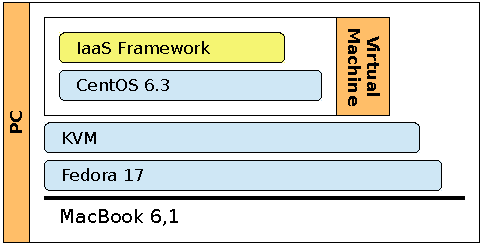
\includegraphics[width=0.55\textwidth]{imagenes/007.pdf}
 \caption{Espacio general de prueba}
\label{fig:espacioprueba}
\end{center}
\end{figure}

\section{Frameworks evaluados}\label{sec:frameworksevaluados}
\hyphenation{CloudStack}
\hyphenation{Eucalyptus}
\hyphenation{OpenNebula}
\hyphenation{OpenStack}
\noindent Los frameworks comparados son:
\begin{itemize}
 \item CloudStack %3.0.2
 \item Eucalyptus %3.1.1
 \item OpenNebula %3.8.1
 \item OpenStack
\end{itemize}

Desde el punto de vista meramente funcional, los cuatro cubren con cla\-ri\-dad la necesidad requerida por el proyecto. A vista de p\'ajaro se requiere la habilidad de gestionar la ejecuci\'on de un n\'umero indeterminado de m\'aquinas virtuales, hechas a medida para MapReduce, a trav\'es de un API que permita definir una sencilla interfaz de control.\newline

Eucalyptus y OpenStack se aproximan a la soluci\'on de forma m\'as mo\-du\-lar, dejando al descubierto partes de funcionalidad m\'as peque\~na, al tiempo que desacoplan esos m\'odulos. As\'i los componentes, se dan instalaciones m\'as flexibles y tediosas a la par, ya que es necesario configurar m\'as m\'odulos por separado. Sin embargo, en OpenStack es posible contener el aumento de esfuerzo utilizando sus scripts de gesti\'on. En cuanto a requisitos operativos, todos soportan \'ultimas o pen\'ultimas versiones de las principales distribuciones de sistemas operativos Linux, y tanto KVM como Xen como hipervisor. En un despliegue sobre una instalaci\'on de un cl\'uster real, la elecci\'on depender\'a m\'as de la plataforma ya configurada que de las limitaciones que pudiese tener el framework concreto.\newline

Como comentario final, decir que la interoperabilidad es la asignatura pendiente a nivel general. Todos se acercan en distinta medida al API de los AWS ---unos lo implementan, otros lo adaptan. OpenNebula, OpenStack y Eucalyptus han demostrado esfuerzos por adherirse al API propuesto desde el Open Grid Forum, que pretende convertirse en el primer API est\'andar (OCCI).\\


%\subsection{Eucalyptus}\label{subsec:eucaliptus}

Eucalyptus, a pesar de haber sido el primero en cubrir el API de los AWS, lo cual es anecd\'otico a estas alturas, presenta dos obst\'aculos para su evaluaci\'on. Primero, no todo el c\'odigo es abierto: el m\'odulo \texttt{VMware Broker}, que abre la puerta a la virtualizaci\'on basada en tecnolog\'ia de VMware, s\'olo est\'a disponible en la versi\'on para suscriptores. Y segundo, no es posible instalar los componentes de Eucalyptus en una m\'aquina virtual como bien describe la gu\'ia de instalaci\'on \cite{eucainstall}. Estos dos obst\'aculos motivan la ca\'ida de Eucalyptus de la lista de evaluaci\'on. El resto de los frameworks han sido evaluados tras su instalaci\'on y configuraci\'on.


\subsection{CloudStack}\label{subsec:cloudstack}

\noindent En \cite{cloudstackquickinstall} se describe la instalaci\'on r\'apida de la \'ultima versi\'on de CloudStack bajo la tutela exclusiva de Citrix. Claramente determina que los nodos de cloud tienen que soportar, como para Eucalyptus, extensiones de vir\-tua\-li\-za\-ci\'on hardware (VT-x o AMD-V) para poder arrancar m\'aquinas virtuales sobre \emph{XenServer} o KVM. Sin embargo, la importancia de que CloudStack pasar\'ia a formar parte de \emph{The Apache Software Foundation} a partir de la versi\'on 4 como proyecto en incubaci\'on \cite{cloudstackstrategy}, y la realidad de un art\'iculo t\'ecnico de Citrix que abr\'ia la puerta a despliegues sobre anfritriones sin extensiones de virtualizaci\'on hardware \cite{cloudstacknohvm} ---a pesar de que incluso el manual de instalaci\'on de CloudStack 4 \cite{apachecloudstack4} siga contemplando esa limitaci\'on---, hizo que se ajustase el entorno de ejecuci\'on de la figura \ref{fig:cloudstack}.\newline

\begin{figure}[tbp]
\begin{center}
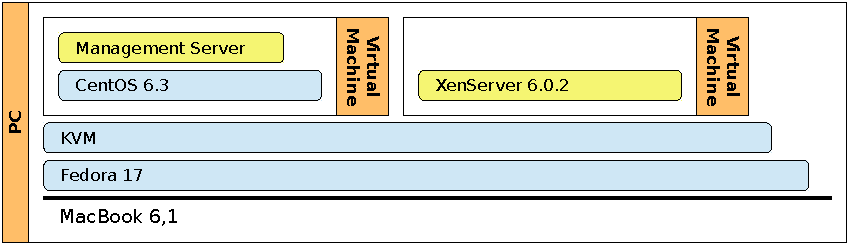
\includegraphics[width=0.99\textwidth]{imagenes/008.pdf}
 \caption{CloudStack 3.0.2 con XenServer como hipervisor}
\label{fig:cloudstack}
\end{center}
\end{figure}

Siguiendo las gu\'ias de instalaci\'on r\'apida y avanzada ---\cite{cloudstackquickinstall} y \cite{cloudstackadvinstall} res\-pec\-ti\-va\-men\-te---, el proceso se puede resumir en los pasos siguientes:

\begin{itemize}
 \item Se crearon dos m�quinas virtuales para contener el \emph{Management Server} (\emph{MS}) de CloudStack y el hipervisor XenServer: 1 GB RAM para el MS, 3 GB RAM para Xen y 20 GB HDD, \emph{ACPI} y \emph{APIC} para ambos.
 \item Para el MS:
  \begin{itemize}
      \item Se descarg\'o, instal\'o y actualiz\'o \emph{CentOS 6.3}.
   \item Se nombr\'o \emph{cloudstack} a la m\'aquina virtual.
   \item Igualmente nombrado, se dio de alta un nuevo usuario, \emph{cloudstack}, y se agreg\'o a la lista de \emph{sudoers}.
   \item Se sigui\'o la gu\'ia de instalaci\'on \cite{cloudstackquickinstall} para concluir el proceso.
  \end{itemize}
 \item Para Xen:
  \begin{itemize}
   \item Se descarg\'o la versi\'on 6.0.2 de XenServer desde la web de Citrix.
   \item Se siguieron los apuntes de la gu\'ia de instalaci\'on de CloudStack \cite{cloudstackquickinstall} y el manual de configuraci\'on de XenServer \cite{xenserverinstall} para realizar la instalaci\'on.
  \end{itemize}
 \item Adicionalmente:
  \begin{itemize}
   \item Antes de crear la zona de ejecuci\'on y definir el cl\'uster, el almacenamiento primario y secundario, etc., se tuvo que modificar la opci\'on de configuraci\'on global para permitir anfitriones sin extensiones de virtualizaci\'on hardware \cite{cloudstacknohvm}.
   \item Una vez verificado el correcto reconocimiento de la infraestructura:
    \begin{itemize}
     \item Se copi\'o la imagen de CentOS 6.3 al MS.
     \item Se arranc\'o un \texttt{SimpleHTTPServer} en el puerto \texttt{443} del MS.
     \item Se permiti\'o el acceso al puerto \texttt{443}, desde \texttt{iptables}, en el MS.
     \item Se carg\'o la imagen en el cloud desde la interfaz web.
    \end{itemize}
  \end{itemize}
\end{itemize}


\subsection{OpenNebula}\label{subsec:opennebula}
\noindent En comparaci\'on con el procedimiento anterior, el esfuerzo de instalaci\'on de OpenNebula 3.8 es muy inferior. De \cite{centosonquickstart} se deriva el proceso que se sigui\'o para configurar el entorno de ejecuci\'on mostrado en la figura \ref{fig:opennebula}, y que se resume en la lista siguiente:

\begin{figure}[tbp]
\begin{center}
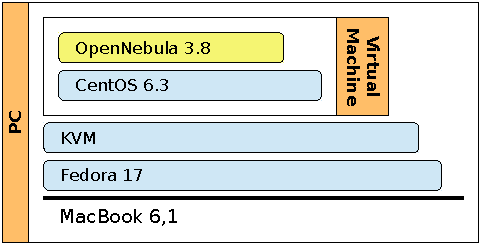
\includegraphics[width=0.55\textwidth]{imagenes/009.pdf}
 \caption{OpenNebula 3.8 con KVM}
\label{fig:opennebula}
\end{center}
\end{figure}

\begin{itemize}
 \item Se cre\'o una m\'aquina virtual soporte para todo el cloud OpenNebula: 1 GB RAM, 8 GB HDD, ACPI y APIC.
 \item Se descarg\'o, instal\'o y actualiz\'o CentOS 6.3.
 \item Se nombr\'o \emph{opennebula} a la m�quina virtual.
 \item Igualmente nombrado, se dio de alta un nuevo usuario, \emph{opennebula}, y se agreg\'o a la lista de \emph{sudoers}.
 \item Se detuvo \texttt{SELinux}.
 \item Se sigui\'o la gu\'ia contenida en \cite{centosonquickstart} para concluir el proceso, al que hubo que integrar las siguientes cuestiones para probar el framework:
  \begin{itemize}
   \item Por defecto, el servicio que brinda la interfaz web de OpenNebula (\texttt{sunstone}) se engancha en \emph{lo}. Para que pudiera ser accedido desde fuera del servidor, fuera de la m\'aquina virtual en este caso, fue necesario precisar que sunstone habr\'ia de escuchar en \emph{eth0}, modificando, para este fin, la configuraci\'on correspondiente en \texttt{/etc/one}. Lo mismo aconteci\'o con \texttt{occi}, el servicio REST de control del cloud.
   \item Adicionalmente, se agreg\'o a iptables la regla para no filtrar el tr\'afico en el puerto \texttt{9869}, el de sunstone inicialmente.
  \end{itemize}
\end{itemize}


\subsection{OpenStack}\label{subsec:openstack}
\noindent El caso de OpenStack es llamativo por varias razones. Representa la convergencia entre dos necesidades diferentes: la puramente computacional de la NASA y la orientada al almacenamiento de Rackspace. Complementariamente, tanto Red Hat como Canonical han sumado su aporte bajo la forma de scripts de instalaci\'on y control en el caso de Red Hat, y escribiendo utilidades de despliegue autom\'atico, como \texttt{juju}, en el caso de Canonical.\newline

Como en el caso de OpenNebula, se configur\'o un entorno de ejecuci\'on contenido en una sola m\'aquina virtual. En este caso se eligi\'o a Fedora frente a CentOS y Ubuntu por el soporte comunitario en forma de extensa gu\'ia de instalaci\'on r\'apida \cite{quickstartfedoraos} y por la existencia de herramientas que ace\-le\-ra\-r\'ian sustancialmente el procedimiento. La gu\'ia de instalaci\'on y despligue oficial de OpenStack Folsom \cite{installdeployosfolsom}, est\'a escrita centr\'andose excesivamente en Ubuntu, lo que se tradujo en comandos no aplicables en Fedora. Como \'ultimo comentario previo a la descripci\'on de la puesta en marcha, decir que se probaron dos versiones de OpenStack: \emph{Essex} y \emph{Folsom}. La raz\'on radica en el hecho de que, a pesar de ser Essex la soportada oficialmente por la distribuci\'on (Fedora 17), desde la gu\'ia r\'apida mencionada anteriormente \cite{quickstartfedoraos} se recomendaba usar la \'ultima versi�n de OpenStack disponible ---Folsom a diciembre de 2012---, habilitando un re\-po\-si\-to\-rio de avance a tal fin.\newline

El grado de madurez observado de Folsom frente a Essex es sustancialmente llamativo en la interfaz web: lo que parec\'ia una primera aproximaci\'on para formular comandos de administraci\'on del cloud, evolucion\'o hacia una interfaz mucho m\'as cohesionada con el comportamiento real. El ejemplo si\-guien\-te pone de manifiesto esta idea: en el momento de lanzar instancias para probar el correcto funcionamiento del cloud, se observ\'o que, en caso de existir alg\'un problema de configuraci\'on en el subsistema de red que impidiese que las instancias obtuviesen direcciones IP, \'estas permanec\'ian en un estado que hac\'ia imposible su eliminaci\'on desde la interfaz web. Fue necesario recurrir a la edici\'on de la base de datos y la estructura de ficheros del controlador del cloud, con algunos resultados nefastos como la p\'erdida de informaci\'on de uso de las instancias, para restablecer la coherencia en Essex. El mismo problema se solventa directamente en Folsom (tanto desde la interfaz web como desde la l\'inea de comandos).\newline

Siguiendo el \'indice siguiente se dispuso un entorno de ejecuci\'on id\'entico para sendas versiones (ver figura \ref{fig:openstack}).

\begin{figure}[tbp]
\begin{center}
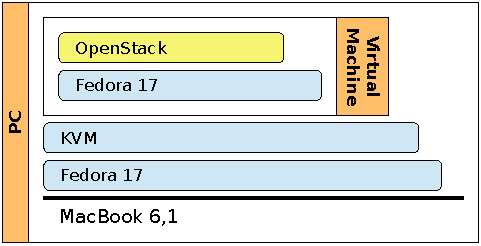
\includegraphics[width=0.55\textwidth]{imagenes/010.pdf}
 \caption{OpenStack en despligue virtual}
\label{fig:openstack}
\end{center}
\end{figure}

\begin{itemize}
 \item Se cre\'o una m\'aquina virtual para todo el cloud OpenStack: 1 GB RAM, 10 GB HDD, APIC y ACPI.
 \item Se descarg\'o, instal\'o y actualiz\'o Fedora 17.
 \item Se nombr\'o \emph{openstack} a la m\'aquina virtual.
 \item Igualmente nombrado, se dio de alta un nuevo usuario, \emph{openstack}, y se agreg\'o a la lista de \emph{sudoers}.
 \item Se instal\'o el paquete \texttt{acpid} para poder controlar los aspectos de energ\'ia desde el manejador de cloud.
 \item Se detuvo SELinux.
 \item Se orden\'o una copia en profundidad de la m\'aquina virtual ---tanto configuraci\'on de la m\'aquina como HDD--- para probar Essex y Folsom, y se renombraron convenientemente.
 \item Se siguieron tanto la gu\'ia de instalaci\'on r\'apida extraoficial \cite{quickstartfedoraos}, como la gu\'ia oficial de despliegue \cite{installdeployosfolsom}, dejando de lado la con\-fi\-gu\-ra\-ci\'on de \texttt{Swift}, para concluir el procedimiento.
 \item A mayores, se crearon sendos discos virtuales de 4 GB para albergar los vol\'umenes del almacenamiento de bloque gestionados por \texttt{Compute}, para Essex, y \texttt{Cinder} para Folsom.
\end{itemize}
 

\section{Conclusiones}\label{sec:conclusiones}
\noindent Presentamos, seguidamente, los resultados de la comparaci\'on de los frameworks de IaaS, atendiendo a las cuestiones resaltadas en la metodolog\'ia.
 
\begin{description}
 \item[Instalaci\'on:] Sin lugar a dudas OpenNebula se lleva la palma. La gu\'ia de instalaci�n es, con mucho, la m\'as corta y ligera de seguir. Acarrea, no obstante, el problema de tener un desconocimiento mayor de lo que est\'a sucediendo bajo la superficie, que dificultar\'a la resoluci\'on de los problemas que pudieran aparecer, as� como el manejo general del cloud.
 \item[Configuraci\'on y manejo:] El aprovisionamiento de nueva infraestructura, es decir, la uni\'on de nuevos anfitriones al cloud, requiere, en todos los frameworks analizados, la instalaci\'on en cada anfitri\'on del hipervisor que se pretenda utilizar. CloudStack y OpenNebula ofrecen una gesti\'on mucho m\'as transparente que OpenStack, siendo necesario ma\-yor esfuerzo de instalaci\'on y configuraci\'on. En este \'ultimo adem\'as, la interfaz web no deja forma alguna de conocer el tama\~no del cl\'uster real sobre el que corre el cloud ni, l\'ogicamente, el grado de utilizaci\'on de la infraestructura. Entre CloudStack y OpenNebula la diferencia es inexistente en cuanto a la funcionalidad expuesta a trav\'es de sus webs. CloudStack expone los servicios de todo el cloud como una jerarqu\'ia; OpenNebula como una tabla.
 \item[Hipervisor:] En cuanto a hipervisores soportados se refiere, OpenStack aventaja claramente a CloudStack y OpenNebula. Sin embargo, se podr\'ia afirmar que este hecho es pr\'acticamente anecd\'otico porque los tres soportan los m\'as conocidos ---KVM, Xen, variantes de Xen y variantes de VMWare--- que son los utilizados en casi todos los despliegues reales.
 \item[Almacenamiento:] Los tres soportan una m\'as que surtida variedad de controladores de \emph{backend} de datos. Pero, en este caso, es importante subrayar el esfuerzo de OpenStack por implementar la funcionalidad ofrecida por Amazon S3 ---almacenamiento en cloud r\'apido y seguro. Swift es el componente de OpenStack que otorga almacenamiento tolerante a fallos y de alta disponibilidad a los despliegues, sustent\'andose para lograrlo en la replicaci\'on y el balanceo de carga, entre otros. La gu\'ia avanzada de instalaci\'on de CloudStack \cite{cloudstackadvinstall}, muestra una primera aproximaci\'on para la configuraci\'on de Swift como almacenamiento secundario del cloud. De ah\'i se puede deducir en cierto grado la importancia y madurez de Swift como m\'odulo de OpenStack.
 \item[Documentaci\'on:] Ninguno de los tres puede presumir de manuales de instalaci\'on oficiales correctos al 100\%. Adem\'as, como se da la circunstancia de que cada framework ha ido madurando con grados de exposici\'on diferentes a las diversas distribuciones Linux, la cobertura que ofrecen para cada sistema operativo es muy heterog\'enea; hasta el punto de confundir, en alg\'un caso, los nombres de los m\'odulos cuyas funciones hay que invocar. Por ejemplo, ambos manuales de instalaci\'on de CloudStack ---r\'apida \cite{cloudstackadvinstall} y avanzada \cite{cloudstackquickinstall}--- se siguen m\'as correctamente usando CentOS como sistema operativo de base y XenServer como hipervisor. OpenStack dispone oficialmente de manuales de ins\-ta\-la\-ci\'on que soportan tanto derivados de Red Hat ---Fedora, CentOS, el propio Red Hat Enterprise Linux, etc.--- como de Debian ---Ubuntu, Debian, etc.--- sin embargo, al realizar el despliegue sobre Fedora se observ\'o que el nombre de los servicios documentados no se correspond\'ia con el nombre real; en Ubuntu no sucede tal cosa. De todas formas, las incorrecciones son nimias y la extensi\'on de la documentaci\'on es m\'as que suficiente para despliegues en producci\'on.
 \item[Comunidad:] A pesar de que pueda resultar algo secundario, la calidad del soporte comunitario es vital para el desarrollo y soporte de los frameworks. Todos ellos est\'an compuestos por m\'odulos escritos en c\'odigo abierto y libre en su mayor parte, de forma que, cuanto mayor sea el bullicio recogido en foros de desarrollo, mayor ser\'a tambi\'en el aporte recibido; y as\'i, el grado de madurez operativo, funcional y documental ser\'a mayor. A pesar de que no pueda darse un claro vencedor en este apartado, debido al car\'acter difuso de la magnitud \emph{soporte comunitario}, s\'i es interesante destacar el importante apoyo a OpenStack de Canonical y Red Hat: no hay conferencia o charla t\'ecnica general de uno u otro donde no hagan referencia a OpenStack.
\end{description}

\subsection{OpenStack Folsom}\label{subsec:openstackfolsom}
\noindent Finalmente, el framework para cloud IaaS elegido es OpenStack Folsom. Las gu\'ias de instalaci\'on mencionadas, el soporte comunitario, el empuje por parte de dos pesos pesados del software, los despliegues reales de HP, Dell, Intel, Rackspace, etc., la modularidad de configuraci\'on, la completitud de implementaci\'on (soporte de los APIs OCCI, S3, EC2 y definici\'on de un servicio de almacenamiento en cloud como Swift) y el soporte oficial de despliegue de prueba sobre m\'aquinas virtuales ---usando emulaci\'on--- han desequilibrado la balanza a su favor.
